\documentclass[10pt]{beamer}

\usetheme{metropolis}
\usepackage{appendixnumberbeamer}
\usepackage{booktabs}
\usepackage{pgfplots}
\usepgfplotslibrary{dateplot}
\usepackage{xspace}
\usepackage{amsmath}
\usepackage{tikz}
\usetikzlibrary{arrows.meta, positioning, fit, backgrounds, decorations.pathreplacing}

% Colors
\definecolor{arcblue}{HTML}{3B82F6}
\definecolor{mathgreen}{HTML}{10B981}
\definecolor{codeorange}{HTML}{F59E0B}
\definecolor{dimgray}{HTML}{9CA3AF}
\definecolor{lightgray}{HTML}{F3F4F6}

\title{PS Generalization: Math \& Code}
\subtitle{mem2 case study --- concept memory across three domains}
\date{February 28, 2026}
\author{}
\institute{}

\begin{document}

\maketitle

% ═════════════════════════════════════════════════════════
\section{Setup}

\begin{frame}{Dataset \& Pipeline Configuration}
  \begin{table}
    \scriptsize
    \begin{tabular}{@{} l ccc @{}}
      \toprule
      & \textcolor{arcblue}{\textbf{ARC-AGI}} & \textcolor{mathgreen}{\textbf{Math L5}} & \textcolor{codeorange}{\textbf{LCB}} \\
      \midrule
      Source & ARC-AGI-1 & competition\_math & release v5+v6 \\
      Build / Eval / Held-out & 400/100/--- & 500/200/1456 & 500/100/--- \\
      Build solve rate & --- & 50\% (Qwen-7B) & 85.5\% (GPT-5m) \\
      Extraction model & GPT-4.1 & Qwen 3.5+ & Qwen 3.5+ \\
      Selection model & GPT-4.1 & Qwen 3.5+ & Qwen 3.5+ \\
      Inference model & GPT-4.1 & Qwen-2.5-7B & Qwen3-Coder \\
      \midrule
      Stage 1 mode & \texttt{code} & \texttt{passthrough} & \texttt{code} \\
      Concepts extracted & 270 & 695 & 341 \\
      \bottomrule
    \end{tabular}
  \end{table}

  \vspace{0.3em}
  Math eval: all 7 MATH categories, Level 5, integer-answer only.\\
  Math split: seed=42 random from 2{,}156 eligible problems.
\end{frame}

% ═════════════════════════════════════════════════════════
\section{Extracted Concepts}

\begin{frame}{Kind Distribution \& Statistics}
  \begin{columns}[T]
    \column{0.58\textwidth}
    \begin{table}
      \tiny
      \begin{tabular}{@{} l r | l r | l r @{}}
        \toprule
        \multicolumn{2}{c|}{\textcolor{arcblue}{\textbf{ARC (270)}}}
        & \multicolumn{2}{c|}{\textcolor{mathgreen}{\textbf{Math (695)}}}
        & \multicolumn{2}{c}{\textcolor{codeorange}{\textbf{Code (341)}}} \\
        \midrule
        routine & 240 & technique & 349 & technique & 280 \\
        structure & 30 & strategy & 210 & algorithm & 35 \\
         & & theorem & 111 & data\_struct & 18 \\
         & & definition & 16 & definition & 8 \\
         & & comp.~strat. & 9 & & \\
        \bottomrule
      \end{tabular}
    \end{table}

    \column{0.38\textwidth}
    \begin{table}
      \tiny
      \begin{tabular}{@{} l rrr @{}}
        \toprule
        & ARC & Math & Code \\
        \midrule
        Concepts & 270 & 695 & 341 \\
        Mean cues & 2.3 & 2.9 & 2.0 \\
        Mean impl & 1.7 & 2.1 & 1.8 \\
        Has params & 89\% & 25\% & 30\% \\
        Max cues & 12 & 32 & 9 \\
        Max used & 96 & 24 & 7 \\
        \bottomrule
      \end{tabular}
    \end{table}
  \end{columns}

  \vspace{0.5em}
  {\footnotesize ARC: 2 kinds (typed routines). Math: 5 kinds. Code: 4 kinds.\\
  ARC: richer params (89\%). Math/Code: longer cues, lower param rate.}
\end{frame}

\begin{frame}{Most-Used Concepts}
  \begin{table}
    \scriptsize
    \begin{tabular}{@{} l l r r r @{}}
      \toprule
      Domain & Concept & Used & Cues & Impl \\
      \midrule
      \textcolor{arcblue}{ARC} & \texttt{extract objects} & 96 & 0 & 0 \\
      & \texttt{recolor object} & 60 & 10 & 6 \\
      & \texttt{draw object} & 48 & 6 & 1 \\
      & \texttt{create new grid} & 48 & 5 & 3 \\
      \midrule
      \textcolor{mathgreen}{Math} & Integer Enumeration in Interval & 24 & 14 & 46 \\
      & Vieta's Formulas & 17 & 32 & 28 \\
      & Divisibility Constraint Propagation & 14 & 24 & 27 \\
      & Positional Base Expansion & 14 & 21 & 22 \\
      \midrule
      \textcolor{codeorange}{Code} & Combin.~Count via Precomp Factorials & 7 & 7 & 8 \\
      & Coordinate Compression & 5 & 8 & 7 \\
      & Offline Query Processing w/ Sorting & 5 & 6 & 7 \\
      & Mod.~Inverse via Fermat's (Precomp) & 5 & 4 & 7 \\
      \bottomrule
    \end{tabular}
  \end{table}

  \vspace{0.3em}
  ARC: high-frequency primitives (96$\times$). Math: moderate reuse with bloat (46 impl). Code: low reuse (max 7).
\end{frame}

\begin{frame}{Concept Example: \textcolor{arcblue}{ARC} --- \texttt{reflect object}}
  \begin{columns}[T]
    \column{0.48\textwidth}
    {\scriptsize
    \textbf{kind}: routine\\
    \textbf{desc}: reflect an object across a specified axis\\
    \textbf{params}: object, axis, mirror\_axis (int|float)\\[0.3em]
    \textbf{cues}:
    \begin{itemize}\setlength\itemsep{0pt}
      \item structures appear with mirrored orientation
      \item reflection relative to a frame, guide, or adjacent pixel
      \item axis determined by position of an indicator or marker
    \end{itemize}
    }

    \column{0.48\textwidth}
    {\scriptsize
    \textbf{implementation}:
    \begin{itemize}\setlength\itemsep{0pt}
      \item use \texttt{np.flip} for standard H/V reflections
      \item calculate mirror axis from reference object position
      \item for each pixel, compute reflected position across axis
    \end{itemize}
    \vspace{0.3em}
    \textbf{used\_in}: 8 problems
    }
  \end{columns}

  \vspace{0.7em}
  \hrule
  \vspace{0.3em}
  {\footnotesize Typed routine: subtype=\texttt{grid manipulation}, output=\texttt{grid|object}. Concrete implementation references (\texttt{np.flip}). Short cues (3). This is the ``good'' case --- compact, actionable.}
\end{frame}

\begin{frame}{Concept Example: \textcolor{mathgreen}{Math} --- Geometric Progression Middle Term}
  \begin{columns}[T]
    \column{0.48\textwidth}
    {\scriptsize
    \textbf{kind}: theorem\\
    \textbf{desc}: for three consecutive GP terms $a, b, c$: $b^2 = ac$\\
    \textbf{params}: (none)\\[0.3em]
    \textbf{cues}:
    \begin{itemize}\setlength\itemsep{0pt}
      \item problem states three numbers form a geometric progression
      \item need algebraic relationship between sequential terms
      \item unknown common ratio makes direct multiplication difficult
      \item quantity changes by fixed fraction at each step
    \end{itemize}
    }

    \column{0.48\textwidth}
    {\scriptsize
    \textbf{implementation}:
    \begin{itemize}\setlength\itemsep{0pt}
      \item applied $(11{+}d)^2 = 9(29{+}2d)$ to convert GP constraint into solvable quadratic
      \item identified ratio $r{=}3/4$, applied iteratively to find $h_1, h_2, h_3$
      \item applied $b^2 = ac$ to digits of 3-digit number to filter candidates
    \end{itemize}
    \vspace{0.3em}
    \textbf{used\_in}: 3 problems
    }
  \end{columns}

  \vspace{0.7em}
  \hrule
  \vspace{0.3em}
  {\footnotesize No \texttt{params} (pure theorem). Cues describe \emph{observable} problem features. Implementations show \emph{concrete} algebraic steps from actual solved problems. Compact: 4 cues, 3 impl.}
\end{frame}

\begin{frame}{Concept Example: \textcolor{codeorange}{Code} --- Binary Search on Answer}
  \begin{columns}[T]
    \column{0.48\textwidth}
    {\scriptsize
    \textbf{kind}: technique\\
    \textbf{desc}: converts maximization into decision problems (``can we achieve X?'') via monotonicity\\
    \textbf{params}: check\_function (predicate), low/high (ints)\\[0.3em]
    \textbf{cues}:
    \begin{itemize}\setlength\itemsep{0pt}
      \item max value satisfying monotonic condition; direct computation hard but verification feasible
      \item max ratio of two sums; verification via graph algorithms
      \item max capacity within fixed budget; greedy subroutine
    \end{itemize}
    }

    \column{0.48\textwidth}
    {\scriptsize
    \textbf{implementation}:
    \begin{itemize}\setlength\itemsep{0pt}
      \item binary search on distance, calling \texttt{can\_select\_k} for independent set of size $k$
      \item 70 iterations on ratio, transforming edge weights to $b - \text{mid} \cdot c$
      \item wraps cost calc in \texttt{can\_achieve\_capacity}, searches $[0, \text{max\_cap}]$
    \end{itemize}
    \vspace{0.3em}
    \textbf{used\_in}: 4 problems
    }
  \end{columns}

  \vspace{0.7em}
  \hrule
  \vspace{0.3em}
  {\footnotesize Identical schema to ARC/Math. Code-specific: typed params (function signature), implementation references actual function names. Instance-specific impl traces vs.\ ARC's reusable pseudocode.}
\end{frame}

\begin{frame}{Bloat Example: \textcolor{mathgreen}{Math} --- Complementary Counting}
  \scriptsize
  \textbf{kind}: strategy \quad \textbf{used\_in}: 10 problems \quad \textbf{27 cues, 16 implementations}

  \textbf{desc}: calculate set size by subtracting failures from total universe

  \vspace{0.3em}
  \textbf{Cues} (showing 5 of 27):
  \begin{enumerate}\setlength\itemsep{0pt}
    \item problem asks for ``at least one'' or ``at least k'' occurrences
    \item direct enumeration involves complex overlapping conditions
    \item the complement condition is significantly simpler to count
    \item problem asks for count with ``none'' of several attributes
    \item total population size is known and fixed
  \end{enumerate}

  \textbf{Implementations} (showing 3 of 16):
  \begin{enumerate}\setlength\itemsep{0pt}
    \item for range 300--399, counted total (100) and subtracted those with no additional 3s ($9 \times 9 = 81$)
    \item transformed ``maximize cupcakes with no ingredients'' into ``minimize union with $\geq$1 ingredient''
    \item computed Total $-$ $|$Union$|$
  \end{enumerate}

  \vspace{0.3em}
  \hrule
  \vspace{0.2em}
  \footnotesize The 27 cues are near-paraphrases of each other. Compression (8192 token budget) reduces to $\sim$18 --- the overgenericness is real, not truncation. Same pattern: \textbf{Vieta's Formulas} (32 cues, 28 impl), \textbf{Integer Enumeration} (14 cues, 46 impl).
\end{frame}

% ═════════════════════════════════════════════════════════
\section{Math Results}

\begin{frame}{Math: Per-Seed Scores (200 problems, Qwen-2.5-7B)}
  \begin{table}
    \footnotesize
    \begin{tabular}{@{} l cccc c @{}}
      \toprule
      Config & s42 & s43 & s44 & s45 & Mean \\
      \midrule
      Baseline (2 pass) & 117 & 120 & 110 & 108 & 113.8 \\
      CR unfiltered (2 pass) & 114 & 113 & --- & --- & 113.5 \\
      CR filtered $\leq$10 cues (2 pass) & 107 & 108 & --- & --- & 107.5 \\
      \bottomrule
    \end{tabular}
  \end{table}

  \vspace{0.5em}
  \begin{table}
    \footnotesize
    \begin{tabular}{@{} l c c @{}}
      \toprule
      Ensemble (pass 1+2) & Oracle & $\Delta$ vs 4B \\
      \midrule
      4$\times$ Baseline & 144 & --- \\
      2B + 2CR unfilt & 146 & +2 \\
      2B + 2CR filt & \textbf{149} & \textbf{+5} \\
      4B + 2CR unfilt & 149 & +5 \\
      4B + 2CR filt & 150 & +6 \\
      \bottomrule
    \end{tabular}
  \end{table}

  \vspace{0.3em}
  {\footnotesize Filtering hurts individual ($-6$) but helps oracle ($+5$). CR individual $\approx$ baseline.}
\end{frame}

\begin{frame}{Oracle Decomposition}
  \begin{center}
  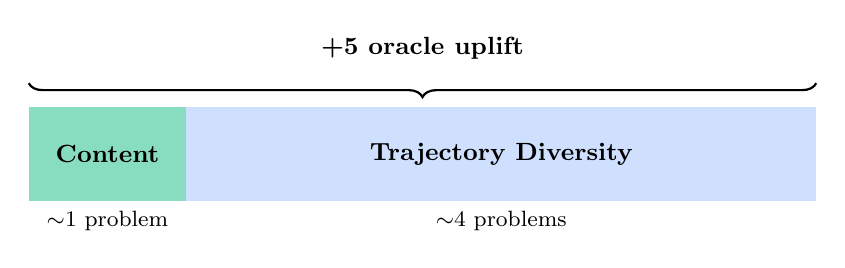
\begin{tikzpicture}
    \fill[arcblue!25] (0,0) rectangle (10,1.2);
    \fill[mathgreen!50] (0,0) rectangle (2,1.2);

    \node[font=\small\bfseries] at (1, 0.6) {Content};
    \node[font=\small\bfseries] at (6, 0.6) {Trajectory Diversity};

    \node[font=\footnotesize, below] at (1, 0) {$\sim$1 problem};
    \node[font=\footnotesize, below] at (6, 0) {$\sim$4 problems};

    \draw[thick, decorate, decoration={brace, amplitude=5pt}]
      (10, 1.5) -- (0, 1.5) node[midway, above=5pt, font=\small\bfseries] {+5 oracle uplift};
  \end{tikzpicture}
  \end{center}

  \vspace{0.5em}
  \begin{table}
    \scriptsize
    \begin{tabular}{@{} l c p{6cm} @{}}
      \toprule
      Category & Count & Evidence \\
      \midrule
      Unique concept pass 2 solve & 1 & cmath\_4005 (complex optimization) --- solved on \emph{both} CR seeds' pass 2, never by any baseline \\
      Apparent harms & 18 & All 18 show False on \emph{both} CR passes --- seed variance, not concept damage \\
      Helped (oracle) & $\sim$19 & Problems solved by CR but not 4B \\
      Hurt (oracle) & $\sim$19 & Problems solved by 4B but not CR --- symmetric \\
      \bottomrule
    \end{tabular}
  \end{table}

  \vspace{0.3em}
  {\footnotesize $\sim$20\% content signal, $\sim$80\% trajectory diversity. Helps and harms cancel.}
\end{frame}

% ═════════════════════════════════════════════════════════
\section{Code Results}

\begin{frame}{LCB: Scores \& Ablation (100 problems, Qwen3-Coder-30B)}
  \begin{table}
    \footnotesize
    \begin{tabular}{@{} l cc @{}}
      \toprule
      Config & s42 & s43 \\
      \midrule
      Baseline & 32 & 35 \\
      Concepts (pass 1+2) & 33 & 40 \\
      \bottomrule
    \end{tabular}
  \end{table}

  \vspace{0.3em}
  \begin{table}
    \footnotesize
    \begin{tabular}{@{} l c c c @{}}
      \toprule
      Ablation (single seed) & $\Delta$ vs base & Helped & Hurt \\
      \midrule
      Composed (cues + filter + route) & +1 & 6 & 5 \\
      Cues-only & $-$1 & 7 & 8 \\
      Filtered (max\_freq=0.3) & $-$5 & 5 & 10 \\
      \bottomrule
    \end{tabular}
  \end{table}

  \vspace{0.5em}
  {\footnotesize All configs within $\pm$5\% of baseline. Indistinguishable from noise at $N{=}100$.\\
  Same pattern as math: helps $\approx$ hurts, net $\approx$ 0.}
\end{frame}

% ═════════════════════════════════════════════════════════
\section{Diagnosis}

\begin{frame}{Why Content Signal is Marginal on Math/Code}
  \textbf{1. Models already know these techniques}

  {\scriptsize Qwen-2.5-7B solves 57\% of L5 math without hints. Vieta's, Complementary Counting, Binary Search on Answer = standard curriculum. Unlike ARC routines, they don't teach something new.}

  \vspace{0.3em}
  \textbf{2. Over-generic concepts on broad datasets}
  \begin{table}
    \scriptsize
    \begin{tabular}{@{} l rrr @{}}
      \toprule
      Concept (Math) & Cues & Impl & Used \\
      \midrule
      Vieta's Formulas & 32 & 28 & 17 \\
      Complementary Counting & 27 & 16 & 10 \\
      Divisibility Constraint Prop. & 24 & 27 & 14 \\
      Integer Enumeration in Interval & 14 & 46 & 24 \\
      \bottomrule
    \end{tabular}
  \end{table}

  \vspace{0.3em}
  {\small \textbf{3. Helps $\approx$ Hurts}}

  {\scriptsize Oracle: $\sim$19 helped, $\sim$19 hurt, net $\approx$ 0. Concepts perturb existing knowledge.}
\end{frame}

\begin{frame}{What Generalizes, What Doesn't}
  \begin{table}
    \scriptsize
    \begin{tabular}{@{} p{5cm} c @{}}
      \toprule
      & Verdict \\
      \midrule
      Pipeline architecture (10 protocols) & \checkmark \\
      Concept schema (fields, merge, render) & \checkmark \\
      Two-stage extraction & \checkmark \\
      Kind taxonomy emerges organically & \checkmark \\
      Stage 1 mode adaptation (code/passthrough) & \checkmark \\
      \midrule
      Content signal on individual scores & $\approx$0 \\
      Concept-retry $>$ always-on & \checkmark \\
      Ensemble diversity from CR & +5 oracle \\
      \midrule
      Content $>$ diversity in oracle uplift & $\times$ (20/80) \\
      Concepts teach model something new & $\times$ \\
      \bottomrule
    \end{tabular}
  \end{table}

  {\footnotesize The \emph{system} generalizes. The \emph{signal} doesn't --- math/code concepts encode standard knowledge.}
\end{frame}

% ═════════════════════════════════════════════════════════
\section{What's Next}

\begin{frame}{Open Questions \& Next Runs}

  \textbf{Model tier upgrade} --- does PS help a strong reasoner?
  \begin{table}
    \scriptsize
    \begin{tabular}{@{} l r l @{}}
      \toprule
      Model & Math L5 Score & Notes \\
      \midrule
      Qwen-2.5-7B & 114/200 (57\%) & Current inference model \\
      GPT-5-mini & 171/200 (85.5\%) & Build run complete, eval pending \\
      \bottomrule
    \end{tabular}
  \end{table}

  \vspace{0.5em}
  \textbf{Verifier/ensembler framing} --- don't gate hints, harvest diversity:
  \begin{itemize}\setlength\itemsep{2pt}
    \item Run baseline + CR, pick best answer via verifier
    \item Oracle ceiling: 149--150/200 (vs 144 baseline oracle)
    \item Agnostic to concept quality
  \end{itemize}

  \vspace{0.5em}
  \textbf{Extraction quality} --- reduce bloat:
  \begin{itemize}\setlength\itemsep{2pt}
    \item Anti-bloat naming rules (v2 prompts, implemented)
    \item Selection running now: Math 200 + LCB 100 (Qwen 3.5+, 600s timeout)
    \item SkillRL-style lean format: title, principle, when\_to\_apply
  \end{itemize}
\end{frame}

% ═════════════════════════════════════════════════════════

\begin{frame}[standout]
  Questions?
\end{frame}

\end{document}
